\section{Introduction}
Community detection is an important topic in graph mining. By learning node community labels on the graph, we are able to detect node hidden attributes as well as explore the closeness between nodes \cite{fortunato2010community}. Conventional methods are mostly user-independent to detect communities solely relying on graph topological structure \cite{fortunato2016community}, generate semi-supervised communities with node constraints \cite{jin2019graph}, or select top-K sub graphs as user-centric communities \cite{li2015influential}. These approaches are no longer enough to satisfy users with a pursuit of personalization, which makes involving user need into community detection to become an inevitable task. Specifically, from a user-centric viewpoint, the ideal communities should provide a high-resolution partition in areas of the graph relevant to the user need and a coarse manner partition on the remaining areas so as to best depict user need (\textit{we also call it ``query'' in the rest of this paper}) in concentrated areas while fuzz irrelevant areas.  

For instance, in Figure \ref{fig:example}, two different scholars in \textit{education} and \textit{data mining} domains may consume the same scholarly graph differently because they may need more detailed community exploration in their own domains while generalized community information in other irrelevant domains (e.g., the \textit{data mining} scholar needs more detailed communities such as \textit{Deep Learning}, \textit{Graph Mining}, and \textit{Bayesian Analysis}.  While an \textit{education} scholar may need to generalize those communities as \textit{Computer Science} or just \textit{Science}). 

\begin{figure}
	% \setlength{\belowcaptionskip}{-10pt}
	\center
	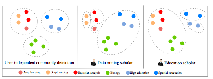
\includegraphics[width=0.8\columnwidth]{img/chapter3/example.pdf} 
	\caption{An example of personalized community detection on a scholarly graph} 
	\label{fig:example}
\end{figure}  

As aforementioned in the Related Work section , current investigations are still with limited scope. First, user-independent approaches solely consider graph topological structure without user need. Second, semi-supervised approaches detect communities restricted by pre-selected seed nodes. As different user needs refer to different seeds, each individual user requires a separate process to run the whole model completely to get personalized communities, which is inapplicable in real cases. Third, sub-graph selection approaches only generate communities from the partial graph instead of the whole one.  

To detect personalized communities on the whole graph, I propose a \textbf{g}enetic \textbf{P}ersonalized \textbf{C}ommunity \textbf{D}etection (gPCD) model with an offline and an online step. Specifically, in the offline step, I convert the user-independent graph community to a binary community tree which is encoded with binary code. Subsequently, a deep learning method is utilized to learn low-dimensional embedding representations for both user need and nodes on the binary community tree. In the online step, I propose a genetic tree-pruning approach on the tree to detect personalized communities by maximizing user need and minimizing user searching cost simultaneously. The whole genetic approach runs in an iterative manner to simulate an evolutionary process and generate a number of partition candidates which are regarded as ``chromosomes'' in each genetic generation. Through the selection, cross-over and mutation process, successive chromosomes are bred as better personalized community partitions to meet with user need.

The contribution of this study is threefold. 
\begin{itemize}
	\item I address a novel personalized community problem and propose a model to generate different-resolution communities associated with user need.   
	\item The proposed model contains an offline and an online step. The offline step takes charge of most calculation to enable an efficient online step: The construction of binary community tree has a time complexity of $O(\rVert V\lVert^{2})$ in the worst case where $\rVert V\lVert$ denotes the number of vertices in the graph; Representation learning on both binary community tree and user need has the same time complexity as Node2vec \cite{grover2016node2vec}. The online genetic pruning step running under the parallel environment achieves $O(\frac{2^dKP}{M})$ time complexity where $d$ denotes the depth of the tree, $K$ denotes the community number, $P$ denotes the initialized population size in the genetic approach and $M$ denotes the number of Mappers/ Reducers in Hadoop Distributed File System (HDFS). 
	\item I evaluate the proposed model on a scholarly graph and a music graph. In my model, the offline step is separately calculated and keeps unchanged once constructed, while the online step guides the personalized community detection. Hence I only compare the online step results with baselines' performance. Extensive experiments shows my model outperforms in terms of both accuracy and efficiency.
\end{itemize}